%% abtex2-modelo-relatorio-tecnico.tex, v-1.9.7 laurocesar
%% Copyright 2012-2018 by abnTeX2 group at http://www.abntex.net.br/ 
%%
%% This work may be distributed and/or modified under the
%% conditions of the LaTeX Project Public License, either version 1.3
%% of this license or (at your option) any later version.
%% The latest version of this license is in
%%   http://www.latex-project.org/lppl.txt
%% and version 1.3 or later is part of all distributions of LaTeX
%% version 2005/12/01 or later.
%%
%% This work has the LPPL maintenance status `maintained'.
%% 
%% The Current Maintainer of this work is the abnTeX2 team, led
%% by Lauro César Araujo. Further information are available on 
%% http://www.abntex.net.br/
%%
%% This work consists of the files abntex2-modelo-relatorio-tecnico.tex,
%% abntex2-modelo-include-comandos and abntex2-modelo-references.bib
%%

% ------------------------------------------------------------------------
% ------------------------------------------------------------------------
% abnTeX2: Modelo de Relatório Técnico/Acadêmico em conformidade com 
% ABNT NBR 10719:2015 Informação e documentação - Relatório técnico e/ou
% científico - Apresentação
% ------------------------------------------------------------------------ 
% ------------------------------------------------------------------------

\documentclass[
	% -- opções da classe memoir --
	12pt,				% tamanho da fonte
	openright,			% capítulos começam em pág ímpar (insere página vazia caso preciso)
	twoside,			% para impressão em recto e verso. Oposto a oneside
	a4paper,			% tamanho do papel. 
	% -- opções da classe abntex2 --
	%chapter=TITLE,		% títulos de capítulos convertidos em letras maiúsculas
	%section=TITLE,		% títulos de seções convertidos em letras maiúsculas
	%subsection=TITLE,	% títulos de subseções convertidos em letras maiúsculas
	%subsubsection=TITLE,% títulos de subsubseções convertidos em letras maiúsculas
	% -- opções do pacote babel --
	english,			% idioma adicional para hifenização
	french,				% idioma adicional para hifenização
	spanish,			% idioma adicional para hifenização
	brazil,				% o último idioma é o principal do documento
	]{abntex2}


% ---
% PACOTES
% ---

% ---
% Pacotes fundamentais 
% ---
\usepackage{lmodern}			% Usa a fonte Latin Modern
\usepackage[T1]{fontenc}		% Selecao de codigos de fonte.
\usepackage[utf8]{inputenc}		% Codificacao do documento (conversão automática dos acentos)
\usepackage{indentfirst}		% Indenta o primeiro parágrafo de cada seção.
\usepackage{color}				% Controle das cores
\usepackage{graphicx}			% Inclusão de gráficos
\usepackage{microtype} 			% para melhorias de justificação
\usepackage{amsmath}
\usepackage{amsfonts}
\usepackage{float}
% ---

% ---
% Pacotes adicionais, usados no anexo do modelo de folha de identificação
% ---
\usepackage{multicol}
\usepackage{multirow}
% ---
	
% ---
% Pacotes adicionais, usados apenas no âmbito do Modelo Canônico do abnteX2
% ---
\usepackage{lipsum}				% para geração de dummy text
% ---

% ---
% Pacotes de citações
% ---
\usepackage[brazilian,hyperpageref]{backref}	 % Paginas com as citações na bibl
\usepackage[alf]{abntex2cite}	% Citações padrão ABNT


% ---
%MINHAS PERSONALIZAÇÕES
% ---
\usepackage{rotating}
\usepackage{booktabs} % Para melhor formatação de tabelas
\usepackage{caption}  % Para customização das legendas
\usepackage[margin=1in]{geometry}
\usepackage{titlesec}


% Redefine o comando de capítulo para não começar em uma nova página
\titleformat{\chapter}[block]
  {\normalfont\huge\bfseries}{\ \ \thechapter}{20pt}{\Huge}
\titlespacing*{\chapter} 
{0pt}{1pt}{1pt}
\titlespacing*{\section}
  {0pt}{1pt}{1pt}
\titlespacing*{\subsection}
  {0pt}{1pt}{1pt}
\titleclass{\chapter}{straight}

\setlength{\intextsep}{10pt}

\setlist[itemize]{noitemsep, topsep=0pt}
\setlength{\abovedisplayskip}{1pt} % espaçamento acima das equações
\setlength{\belowdisplayskip}{1pt} % espaçamento abaixo das equações
\setlength{\abovedisplayshortskip}{1pt} % espaçamento curto acima das equações
\setlength{\belowdisplayshortskip}{1pt} % espaçamento curto abaixo das equações

% Ajuste do espaçamento ao redor do ambiente aligned
\setlength{\abovedisplayshortskip}{1pt}
\setlength{\belowdisplayshortskip}{1pt}


% --- 
% CONFIGURAÇÕES DE PACOTES
% --- 

% ---
% Configurações do pacote backref
% Usado sem a opção hyperpageref de backref
\renewcommand{\backrefpagesname}{Citado na(s) página(s):~}
% Texto padrão antes do número das páginas
\renewcommand{\backref}{}
% Define os textos da citação
\renewcommand*{\backrefalt}[4]{
	\ifcase #1 %
		Nenhuma citação no texto.%
	\or
		Citado na página #2.%
	\else
		Citado #1 vezes nas páginas #2.%
	\fi}%
% ---

% ---
% Informações de dados para CAPA e FOLHA DE ROSTO
% ---
\titulo{Relatório da 4ª prática}
\autor{Romário Jonas de Oliveira Veloso}
\local{Recife - PE}
\data{2024}
\instituicao{%
  Universidade Federal de Pernambuco (UFPE)
  \par
  Centro de Tecnologia e Geociências (CTG)
  \par
  Departamento de Eletrônica e Sistemas (DES)}
\tipotrabalho{Relatório técnico}
% O preambulo deve conter o tipo do trabalho, o objetivo, 
% o nome da instituição e a área de concentração 
\preambulo{Relatório Técnico para a disciplina Circuitos Elétricos 2, período 2024.1.}
% ---

% ---
% Configurações de aparência do PDF final

% alterando o aspecto da cor azul
\definecolor{blue}{RGB}{41,5,195}

% informações do PDF
\makeatletter
\hypersetup{
     	%pagebackref=true,
		pdftitle={\@title}, 
		pdfauthor={\@author},
    	pdfsubject={\imprimirpreambulo},
	    pdfcreator={LaTeX with abnTeX2},
		pdfkeywords={abnt}{latex}{abntex}{abntex2}{relatório técnico}, 
		colorlinks=true,       		% false: boxed links; true: colored links
    	linkcolor=blue,          	% color of internal links
    	citecolor=blue,        		% color of links to bibliography
    	filecolor=magenta,      		% color of file links
		urlcolor=blue,
		bookmarksdepth=4
}
\makeatother
% --- 

% --- 
% Espaçamentos entre linhas e parágrafos 
% --- 

% O tamanho do parágrafo é dado por:
\setlength{\parindent}{1.3cm}

% Controle do espaçamento entre um parágrafo e outro:
\setlength{\parskip}{0.2cm}  % tente também \onelineskip

% ---
% compila o indice
% ---
\makeindex
% ---

% ----
% Início do documento
% ----
\begin{document}

% Seleciona o idioma do documento (conforme pacotes do babel)
%\selectlanguage{english}
\selectlanguage{brazil}

% Retira espaço extra obsoleto entre as frases.
\frenchspacing 

% ----------------------------------------------------------
% ELEMENTOS PRÉ-TEXTUAIS
% ----------------------------------------------------------
% \pretextual

% ---
% Capa
% ---
\imprimircapa
% ---

% ---
% Folha de rosto
% (o * indica que haverá a ficha bibliográfica)
% ---
\imprimirfolhaderosto*
% ---


% ---
% inserir o sumario
% ---
%\pdfbookmark[0]{\contentsname}{toc}
%\tableofcontents*
%\cleardoublepage
% ---


% ----------------------------------------------------------
% ELEMENTOS TEXTUAIS
% ----------------------------------------------------------
\textual



\chapter{Introdução}
Neste laboratório, será projetado e implementado um filtro passivo RC passa-baixa. Serão analisados o comportamento na frequência, com e sem carga, da magnitude de resposta em frequência. Será utilizado um buffer para diminuir o impacto de uma carga no comportamento do circuito.

\chapter{Objetivos Gerais}
Conhecer as características de um circuito RC que se comporta como um filtro passa-baixa e treinar a análise de circuitos com carga e com fontes não-ideais.

\chapter{Objetivos Específicos}
\begin{itemize}
    \item Aplicar a transformada de Laplace na análise de circuitos.
    \item Usar um amplificador operacional como buffer.
    \item Medir as grandezas elétricas em um circuito usando um osciloscópio.
    \item Comparar o comportamento na frequência de circuitos de filtros com o comportamento esperado.
    \item Usar o SymPy para resolver equações algébricas aplicadas na resolução de circuitos elétricos.
\end{itemize}

\clearpage
\chapter{Metodologia}

\section{Equipamentos e Materiais Necessários}
Para a realização desta prática, serão utilizados tanto softwares específicos quanto componentes eletrônicos. Os recursos computacionais incluem:
\begin{itemize}
    \item Jupyter Notebook;
    \item Osciloscópio \cite{keysight_manual};
    \item Fonte de tensão;
    \item Multímetro \cite{keysight-u1250};
\end{itemize}

Com os materiais e softwares preparados, o próximo passo envolve a análise detalhada dos circuitos planejados para esta prática. Esta análise é fundamental para entender as respostas teóricas e práticas dos filtros.

\section{Análise do Circuito}
Esta seção aborda a análise dos três circuitos propostos, explorando suas características e comportamentos em diferentes configurações.

\subsection{Primeiro Circuito: Filtro Passa-Baixa RC Sem Carga}
Este circuito consiste de um simples arranjo RC em série, cuja saída é tomada através do capacitor. O diagrama abaixo ilustra o circuito:

\begin{figure}[H]
\centering
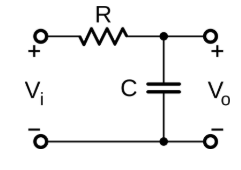
\includegraphics[width=0.5\textwidth]{imgs/first_circuit_diagram.png}
\caption{Diagrama do Primeiro Circuito: Filtro Passa-Baixa RC Sem Carga. (Fonte: \cite{ufpe2023pratica})}
\label{fig:first_circuit_analysis}
\end{figure}

A função de transferência do circuito é descrita pela seguinte equação:
\begin{equation}
    H_1(s) = \frac{\frac{1}{RC}}{s + \frac{1}{RC}}
    \label{eq:first_transfer_function}
\end{equation}

A frequência de corte, \(\omega_c\), é determinada por:
\begin{equation}
    \omega_c = \frac{1}{RC}
    \label{eq:cutoff_frequency}
\end{equation}
\,

\subsubsection{Projeto do Filtro}

Para projetar o filtro de modo que ele tenha ganho unitário e frequência de corte \( f_c = 50 \) Hz, e usando um capacitor de 100 nF, precisamos determinar o valor adequado de \( R \). A frequência de corte \(f_c\) pode ser calculada usando a seguinte fórmula:
\begin{equation}
    f_c = \frac{1}{2\pi RC}
\end{equation}
Substituindo \(f_c = 50\) Hz e \(C = 100\) nF na equação, podemos resolver para \(R\):
\begin{equation}
    R = \frac{1}{2\pi \times 50 \times 100 \times 10^{-9}}
\end{equation}
\begin{equation}
    R \approx \frac{1}{2\pi \times 50 \times 100 \times 10^{-9}} \approx 31.8 \text{ k}\Omega
\end{equation}
Este valor de \(R\) precisa ser ajustado para o valor comercial mais próximo disponível. Considerando os padrões comerciais, o valor de \(33 \text{ k}\Omega\) é uma escolha comum e está disponível nas séries E12 e E24 de resistores. Usando um resistor de \(33 \text{ k}\Omega\), a frequência de corte será ligeiramente ajustada:
\begin{equation}
    \omega_c' = \frac{1}{2\pi \times 33 \times 10^3 \times 100 \times 10^{-9}} \approx 48 \, \text{Hz}
\end{equation}
Este valor ajustado de \(\omega_c'\) ainda está bastante próximo do objetivo de 50 Hz, demonstrando que a alteração é aceitável para a maioria das aplicações práticas.  Conforme descrito na Equação~\ref{eq:transfer_function}, a análise de resposta em frequência será essencial para determinar o diagrama de Bode de magnitude do filtro.

\subsubsection{Diagrama de Bode do Filtro}
A análise de Bode é essencial para entender o comportamento em frequência do filtro. Os diagramas de Bode de magnitude e fase fornecem uma representação visual da resposta do filtro em frequência e fase ao longo de um intervalo de frequências. Abaixo estão os diagramas de Bode para o filtro RC com um resistor de \(33 \text{ k}\Omega\) e um capacitor de 100 nF.

\begin{figure}[H]
    \centering
    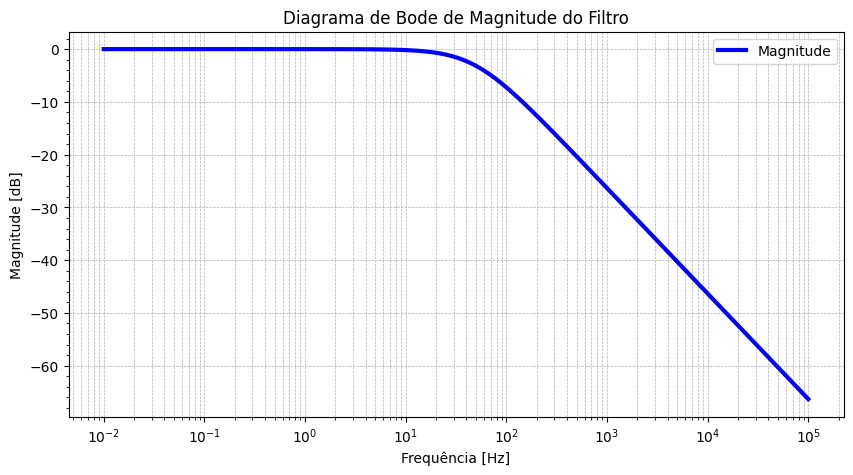
\includegraphics[width=0.85\textwidth]{imgs/first_circuit_bode_magnitude.png}
    \hspace{0.05\textwidth} % Espaçamento entre as imagens
    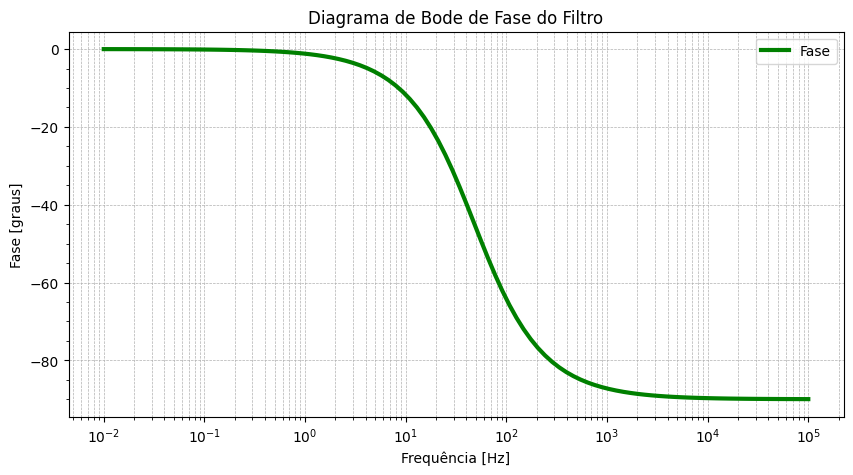
\includegraphics[width=0.85\textwidth]{imgs/first_circuit_bode_phase.png}
    \caption{Acima, o diagrama de Bode de magnitude do filtro. Abaixo, o diagrama de Bode de fase do filtro.}
    \label{fig:first_circuit_bode_diagrams}
\end{figure}



Estes diagramas são fundamentais para a análise detalhada do desempenho do filtro em várias frequências. A magnitude mostra como o filtro atenua ou amplifica diferentes frequências, enquanto o gráfico de fase indica a mudança de fase que cada componente de frequência experimenta ao passar pelo filtro.

\subsubsection{Simulação no LTSpice}
Para complementar a análise analítica e os diagramas de Bode, é realizada uma simulação no software LTSpice \cite{ltspice}. A simulação serve para validar o design do filtro e para observar seu comportamento sob condições operacionais simuladas. A seguir, está apresentado o diagrama do circuito montado no LTSpice para o primeiro circuito.

\begin{figure}[H]
    \centering
    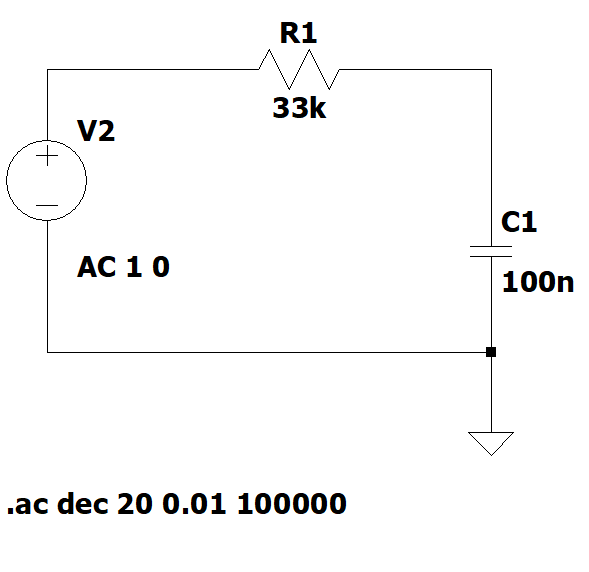
\includegraphics[width=0.5\textwidth]{imgs/first_circuit_ltspice_diagram.png}
    \caption{Diagrama do circuito montado no LTSpice para o primeiro circuito.}
    \label{fig:first_circuit_ltspice_diagram}
\end{figure}

Este diagrama ilustra a configuração do circuito utilizado na simulação, incluindo todos os componentes e conexões necessárias para a análise do filtro RC. Essa visualização ajuda a garantir que o modelo no LTSpice esteja configurado corretamente conforme o design teórico.

\begin{figure}[H]
    \centering
    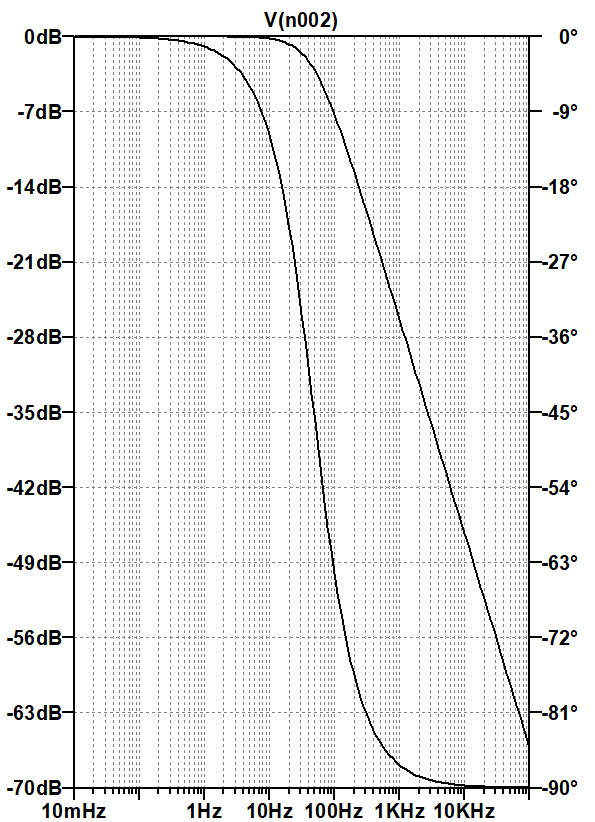
\includegraphics[width=0.8\textwidth,height=0.45\textwidth]{imgs/first_circuit_ltspice_bode.png}
    \caption{Diagrama de Bode do circuito no LTSpice.}
    \label{fig:first_circuit_ltspice_bode}
\end{figure}


O diagrama de Bode gerado pela simulação fornece informações sobre a resposta em frequência do filtro, incluindo a magnitude e a fase. Comparar este diagrama com os resultados analíticos ajuda a identificar qualquer discrepância e a realizar ajustes necessários no design ou na configuração do circuito.


\subsection{Segundo Circuito: Filtro Passa-Baixa RC Com Carga RL}

Adicionando uma carga RL à saída do filtro RC, este circuito explora como a presença da carga afeta as características do filtro, incluindo o ganho e a frequência de corte. A inclusão de \( R_L \) altera a constante de tempo do circuito, modificando assim a função de transferência e a frequência de corte.

\begin{figure}[H]
\centering
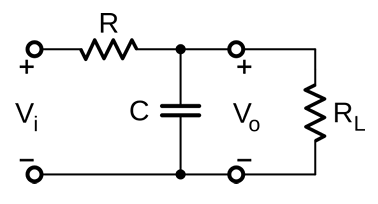
\includegraphics[width=0.5\textwidth]{imgs/second_circuit_diagram.png}
\caption{Diagrama do Segundo Circuito: Filtro Passa-Baixa RC Com Carga RL. (Fonte: \cite{ufpe2023pratica})}
\label{fig:second_circuit_analysis}
\end{figure}

A função de transferência é dada pela seguinte equação, onde \( K \) é um fator de divisão de tensão determinado pela relação entre \( R_L \) e a soma \( R + R_L \):
\begin{equation}
    H_2(s) = \frac{\frac{1}{RC}}{s + \frac{1}{KRC}}
    \label{eq:second_transfer_function}
\end{equation}
onde \( K = \frac{R_L}{R + R_L} \).

A frequência de corte ajustada, \( \omega_c \), é recalculada para refletir o impacto da carga \( R_L \):
\begin{equation}
    \omega_c = \frac{1}{KRC}
    \label{eq:cutoff_frequency_loaded}
\end{equation}


Considerando agora o filtro projetado anteriormente com \( R = 33 \, k\Omega \), \( C = 100 \, nF \), e uma frequência de corte de \( f_c = 50 \, Hz \), com um resistor de carga \( R_L = 22 \, k\Omega \), a função de transferência é determinada pela fórmula já fornecida. O fator \( K \), que é importante para a frequência de corte e o ganho do circuito, é calculado como:

\begin{equation}
    K = \frac{R_L}{R + R_L} = \frac{22 \, k\Omega}{33 \, k\Omega + 22 \, k\Omega} \approx 0.4
    \label{eq:k_factor_loaded}
\end{equation}

Substituindo \( K \), \( R \), e \( C \) na fórmula da frequência de corte, obtemos:

\begin{equation}
    f_c = \frac{1}{{2\pi}KRC} \approx \frac{1}{0.4 \times {2\pi} \times 33 \times 10^3 \times 100 \times 10^{-9}} \approx 120.5 \, \text{Hz}
    \label{eq:omega_c_loaded}
\end{equation}

Este resultado mostra que a frequência de corte do filtro aumenta para aproximadamente 120.5 Hz quando um resistor de carga \( R_L \) é incluído, indicando a influência significativa da carga sobre o comportamento do filtro.


\subsubsection{Diagrama de Bode do Filtro}

A resposta em frequência do filtro com a nova configuração de \( R \) e \( R_L \) é fundamental para confirmar a eficácia do projeto. Os diagramas de Bode de magnitude e de fase são apresentados a seguir para ilustrar isso:

\begin{figure}[H]  
    \centering
    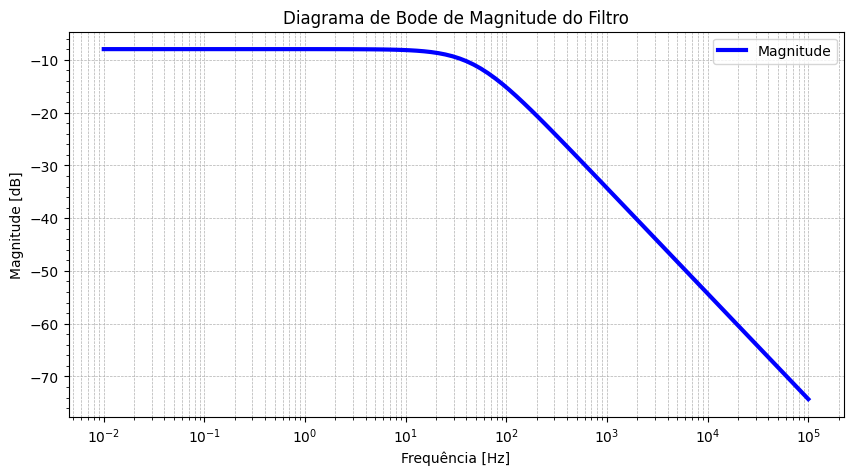
\includegraphics[width=0.85\textwidth]{imgs/second_circuit_bode_magnitude.png}
    \hspace{0.05\textwidth}
    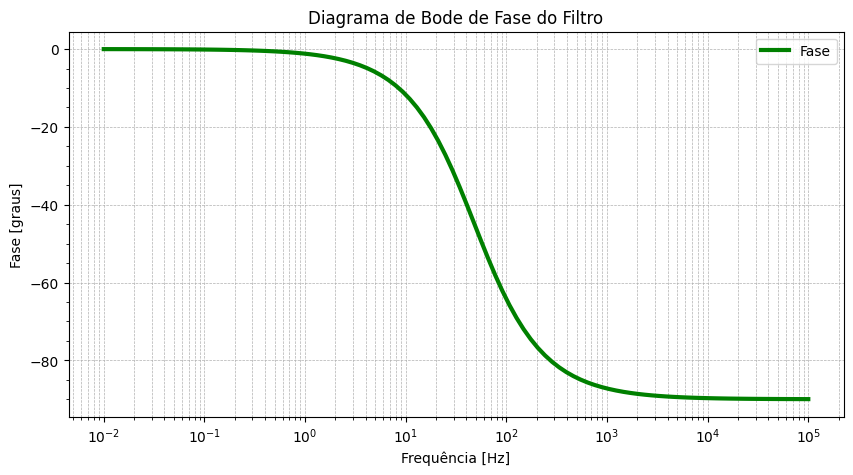
\includegraphics[width=0.85\textwidth]{imgs/second_circuit_bode_phase.png}
    \caption{Acima, o diagrama de Bode de magnitude do segundo circuito. Abaixo, o diagrama de Bode de fase do segundo circuito.}
    \label{fig:second_circuit_bode_diagrams}
\end{figure}

As alterações no ganho e na fase demonstradas nos gráficos são críticas para avaliar as capacidades de atenuação e estabilidade do filtro. Com essa visualização direta da resposta em frequência do filtro, avançaremos para uma validação ainda mais detalhada através da simulação computacional.
\pagebreak

\subsubsection{Simulação no LTSpice}
Para consolidar os dados obtidos e verificar a performance do filtro em condições controladas, foi realizada uma simulação detalhada no software LTSpice. A seguir, é apresentado o diagrama do circuito montado no LTSpice, juntamente com o gráfico do diagrama de Bode gerado pela simulação.

\begin{figure}[H]
    \centering
    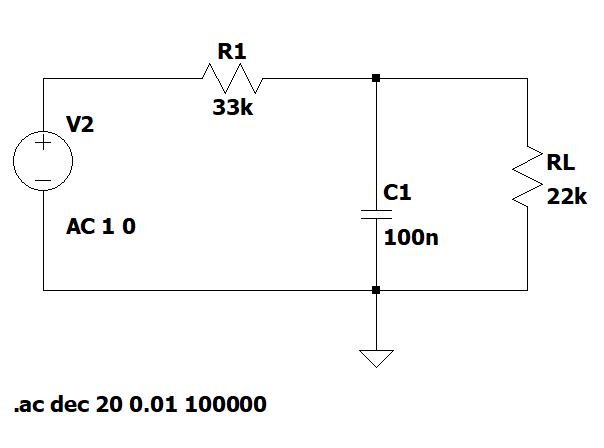
\includegraphics[width=0.6\textwidth]{imgs/second_circuit_ltspice_diagram.png}
    \caption{Diagrama do circuito montado no LTSpice para o segundo circuito.}
    \label{fig:second_circuit_ltspice_diagram}
\end{figure}

O diagrama ilustra detalhadamente o arranjo dos componentes dentro do simulador LTSpice, facilitando a comparação direta com o design teórico. As simulações são fundamentais para garantir que todas as expectativas de projeto se reflitam adequadamente na prática.

\begin{figure}[H]
    \centering    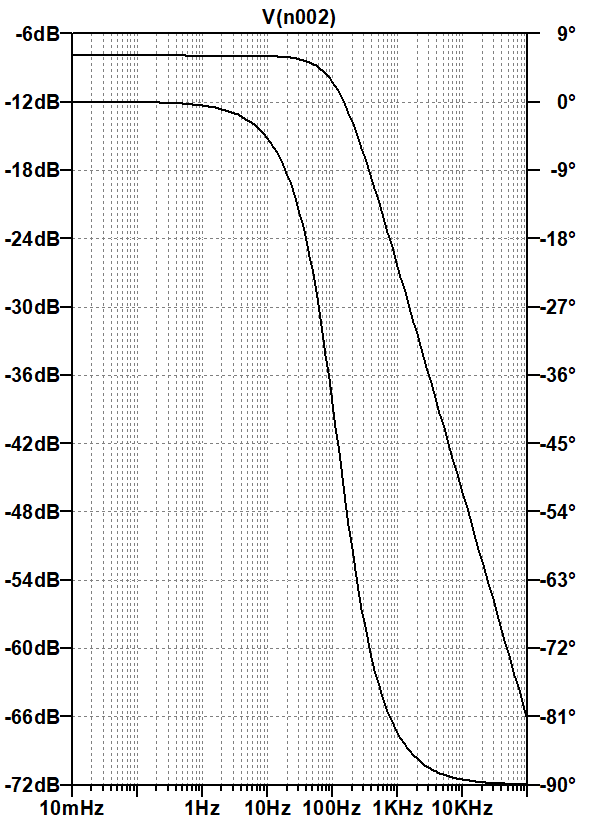
\includegraphics[width=0.7\textwidth,height=0.4\textwidth]{imgs/second_circuit_ltspice_bode.png}
    \caption{Diagrama de Bode do segundo circuito no LTSpice.}
    \label{fig:second_circuit_ltspice_bode}
\end{figure}


Estas simulações confirmam as previsões analíticas e oferecem uma validação adicional de que o filtro opera dentro dos parâmetros esperados.
\pagebreak

\subsection{Terceiro Circuito: Filtro Passa-Baixa RC Com Buffer Ampop}
O terceiro circuito incorpora um buffer amplop seguindo o arranjo básico de um filtro passa-baixa RC. A presença do amplificador operacional configurado como buffer visa minimizar a influência de qualquer carga conectada na saída do filtro sobre a sua função de transferência.

\begin{figure}[H]
\centering
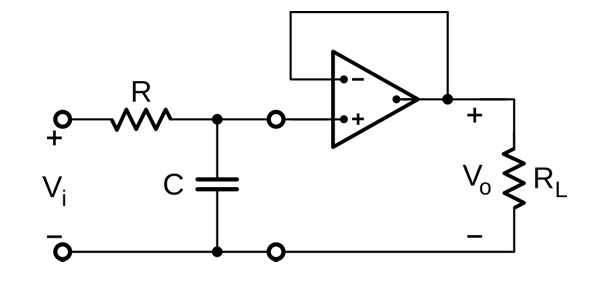
\includegraphics[width=0.7\textwidth]{imgs/third_circuit_diagram.png}
\caption{Diagrama do Terceiro Circuito: Filtro Passa-Baixa RC Com Buffer Ampop. (Fonte: \cite{ufpe2023pratica})}
\label{fig:third_circuit_analysis}
\end{figure}

O circuito equivalente para este filtro, em termos de função de transferência e frequência de corte, é o mesmo que o do Primeiro Circuito (veja Figura~\ref{fig:first_circuit_analysis}). Isso ocorre porque  O buffer é usado para garantir que a carga ($R_L$) não afete a função de transferência do filtro RC. O buffer, sendo ideal, tem uma impedância de entrada infinita e ganho de tensão unitário. Dessa forma, a função de transferência e frequência de corte são as mesmas que as do primeiro circuito, expressas nas Equações~\ref{eq:first_transfer_function} e ~\ref{eq:cutoff_frequency}, respectivamente.

\pagebreak

\subsubsection{Simulação no LTSpice}
Para validar a análise teórica e observar o comportamento do filtro com o buffer, uma simulação detalhada foi realizada no LTSpice. A seguir são apresentados tanto o diagrama do circuito simulado quanto o diagrama de Bode obtido pela simulação.

\begin{figure}[H]
    \centering
    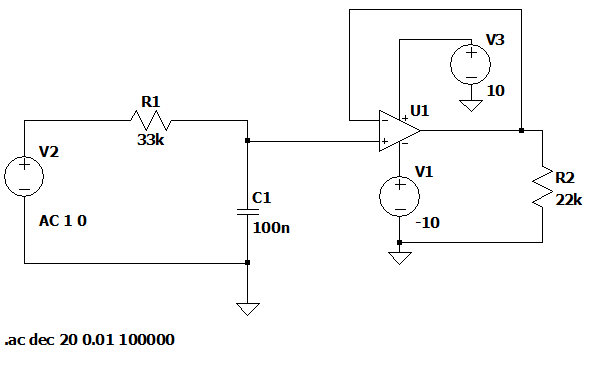
\includegraphics[width=0.5\textwidth]{imgs/third_circuit_ltspice_diagram.png}
    \caption{Diagrama do circuito montado no LTSpice para o Terceiro Circuito.}
    \label{fig:third_circuit_ltspice_diagram}
\end{figure}

Este diagrama mostra claramente como o filtro RC é configurado no LTSpice, incluindo o buffer, o que é crucial para garantir uma simulação precisa.

\begin{figure}[H]
    \centering    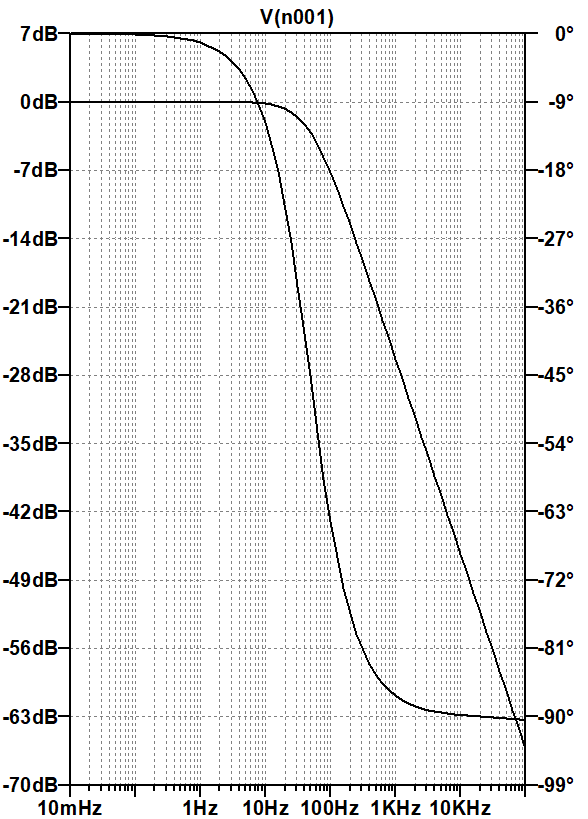
\includegraphics[width=0.5\textwidth,height=0.4\textwidth]{imgs/third_circuit_ltspice_bode.png}
    \caption{Diagrama de Bode do Terceiro Circuito no LTSpice.}
    \label{fig:third_circuit_ltspice_bode}
\end{figure}

O Diagrama de Bode ilustra a resposta em frequência do filtro, confirmando teoricamente as expectativas com uma representação visual precisa das alterações de magnitude e fase ao longo do espectro de frequências.

Com os resultados da simulação fornecendo uma compreensão detalhada da resposta do circuito, a próxima etapa envolve a validação prática destas observações. As medições em laboratório não só confirmam os dados da simulação como também ajudam a identificar qualquer comportamento inesperado dos componentes reais.

\pagebreak

\chapter{Medições em Laboratório}

Para a segunda parte da prática, o circuito será montado em uma protoboard e serão realizadas medições do sinal de saída, comparando-o com a entrada para determinar a diferença de magnitude e fase da entrada para a saída.

\section{Medição dos Componentes com Multímetro}

Utilizando um multímetro, os valores dos resistores e capacitores do circuito serão medidos e registrados. A tabela abaixo compara os valores esperados com os valores mensurados:

\begin{table}[H]
    \small
    \scriptsize
    \centering
    \begin{tabular}{|c|c|c|}
        \hline
        Componente & Valor Esperado & Valor Mensurado \\
        \hline
        Capacitor (C) & 100 nF & 98 nF \\
        Resistor (R) & 33 k\(\Omega\) & 32.7 k\(\Omega\) \\
        Resitor ($R_L$) & 22 k\(\Omega\)  & 21.3 k\(\Omega\) \\
        \hline
    \end{tabular}
    \caption{Comparação dos valores esperados e mensurados dos componentes com multímetro \cite{keysight-u1250}}
    \label{tab:component_values}
\end{table}


\section{Primeiro Circuito}


\subsection{Montagem do Circuito na Protoboard}

O circuito será montado na protoboard. Após a montagem, a fonte de tensão será conectada para alimentar o circuito. A figura abaixo mostra o circuito montado na protoboard.



\subsection{Configuração do Osciloscópio}

O gerador de sinal do osciloscópio será conectado na entrada \( v_i(t) \) do circuito. O gerador será configurado para gerar uma onda senoidal de amplitude de 5 V pico a pico e a frequência será ajustada para a mínima disponível de 100 mHz para observar a máxima tensão de saída que o filtro passa-baixa pode oferecer nas frequências baixas.

\begin{figure}[H]
    \centering
    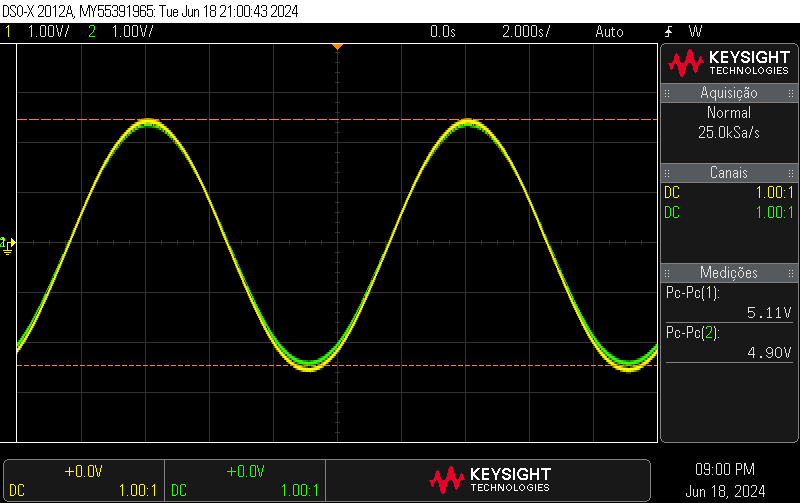
\includegraphics[width=0.6\textwidth]{imgs/first_oscilloscope_low_frequency_output.jpg}
    \caption{Curva de saída no osciloscópio para a frequência mínima de 100 mHz.}
    \label{fig:low_frequency_output}
\end{figure}

\subsection{Cálculo da Tensão Máxima}

Com base na máxima tensão de saída observada de 4.9 V, o valor de \( H_{\text{max}} \) é calculado da seguinte forma:

\begin{equation}
H_{\text{max}} = \frac{1}{\sqrt{2}} \times 4.9 \approx 3.4648 \text{V}
\end{equation}

Este valor será utilizado para análises adicionais.


\subsection{Frequência de Corte Observada}
A frequência de corte observada, onde a amplitude de saída cai para 70.7\% da amplitude máxima observada, foi determinada como 53 Hz (ver Figura \ref{fig:first_oscilloscope_cutoff_frequency}. Esta informação é essencial para validar a performance do filtro em atenuar frequências acima deste ponto.


\begin{figure}[H]
    \centering
    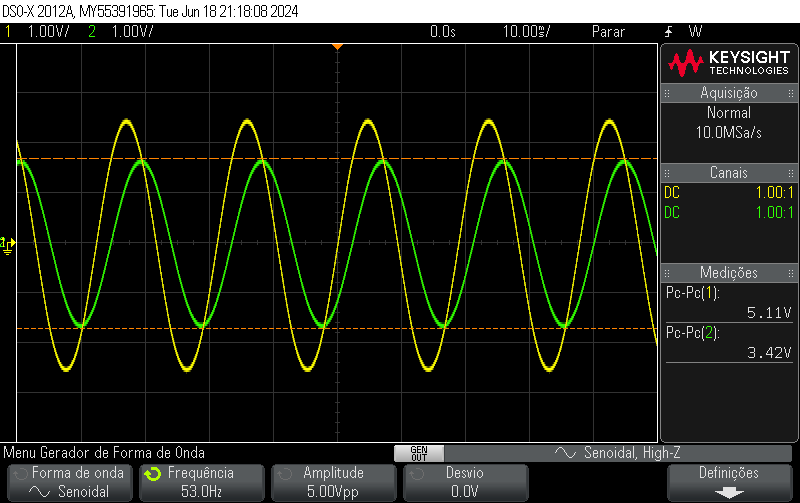
\includegraphics[width=0.75\textwidth]{imgs/first_oscilloscope_cutoff_frequency.jpg}
    \caption{Curva de saída no osciloscópio mostrando a frequência de corte para o Primeiro Circuito.}
    \label{fig:first_oscilloscope_cutoff_frequency}
\end{figure}

Este procedimento assegura uma compreensão detalhada da característica passa-baixa do filtro e da influência da frequência sobre a amplitude do sinal.

\subsection{Medição de Amplitudes em Frequências Variadas}

A amplitude de saída será medida para diferentes frequências para avaliar a frequência de corte do filtro. As amplitudes de entrada e saída para cada frequência testada serão registradas na seguinte tabela:

\begin{table}[H]  
    \centering
    \begin{tabular}{|c|c|c|}
        \hline
        Frequência (Hz) & Amplitude de Entrada (Vi) & Amplitude de Saída (Vo) \\
        \hline
        100 m & 5.11 V & 4.9 V \\
        1.06 & 5.11 V & 4.9 V \\
        10.6 & 5.11 V & 4.78 V \\
        26.5 & 5.11 V & 4.38 V \\
        39.8 & 5.11 V & 3.9 V \\
        53 & 5.11 V & 3.46 V \\
        66.3 & 5.11 V & 3.1 V \\
        84.8 & 5.11 V & 2.61 V \\
        132.5 & 5.11 V & 1.89 V \\
        185.5 & 5.11 V & 1.41 V \\
        265 & 5.11 V & 1.01 V \\
        530 & 5.11 V & 560 mV \\
        1060 & 5.11 V & 360 mV \\
        \hline
    \end{tabular}
    \caption{Amplitudes de entrada e saída para diferentes frequências no circuito 1}
    \label{tab:frequency_response}
\end{table}

Este procedimento assegura uma compreensão detalhada da característica passa-baixa do filtro e da influência da frequência sobre a amplitude do sinal.

\section{Segundo Circuito}

\subsection{Montagem do Circuito na Protoboard}

O circuito será montado na protoboard. Após a montagem, a fonte de tensão será conectada para alimentar o circuito. A figura abaixo mostra o circuito montado na protoboard.

\begin{figure}[H]
    \centering
    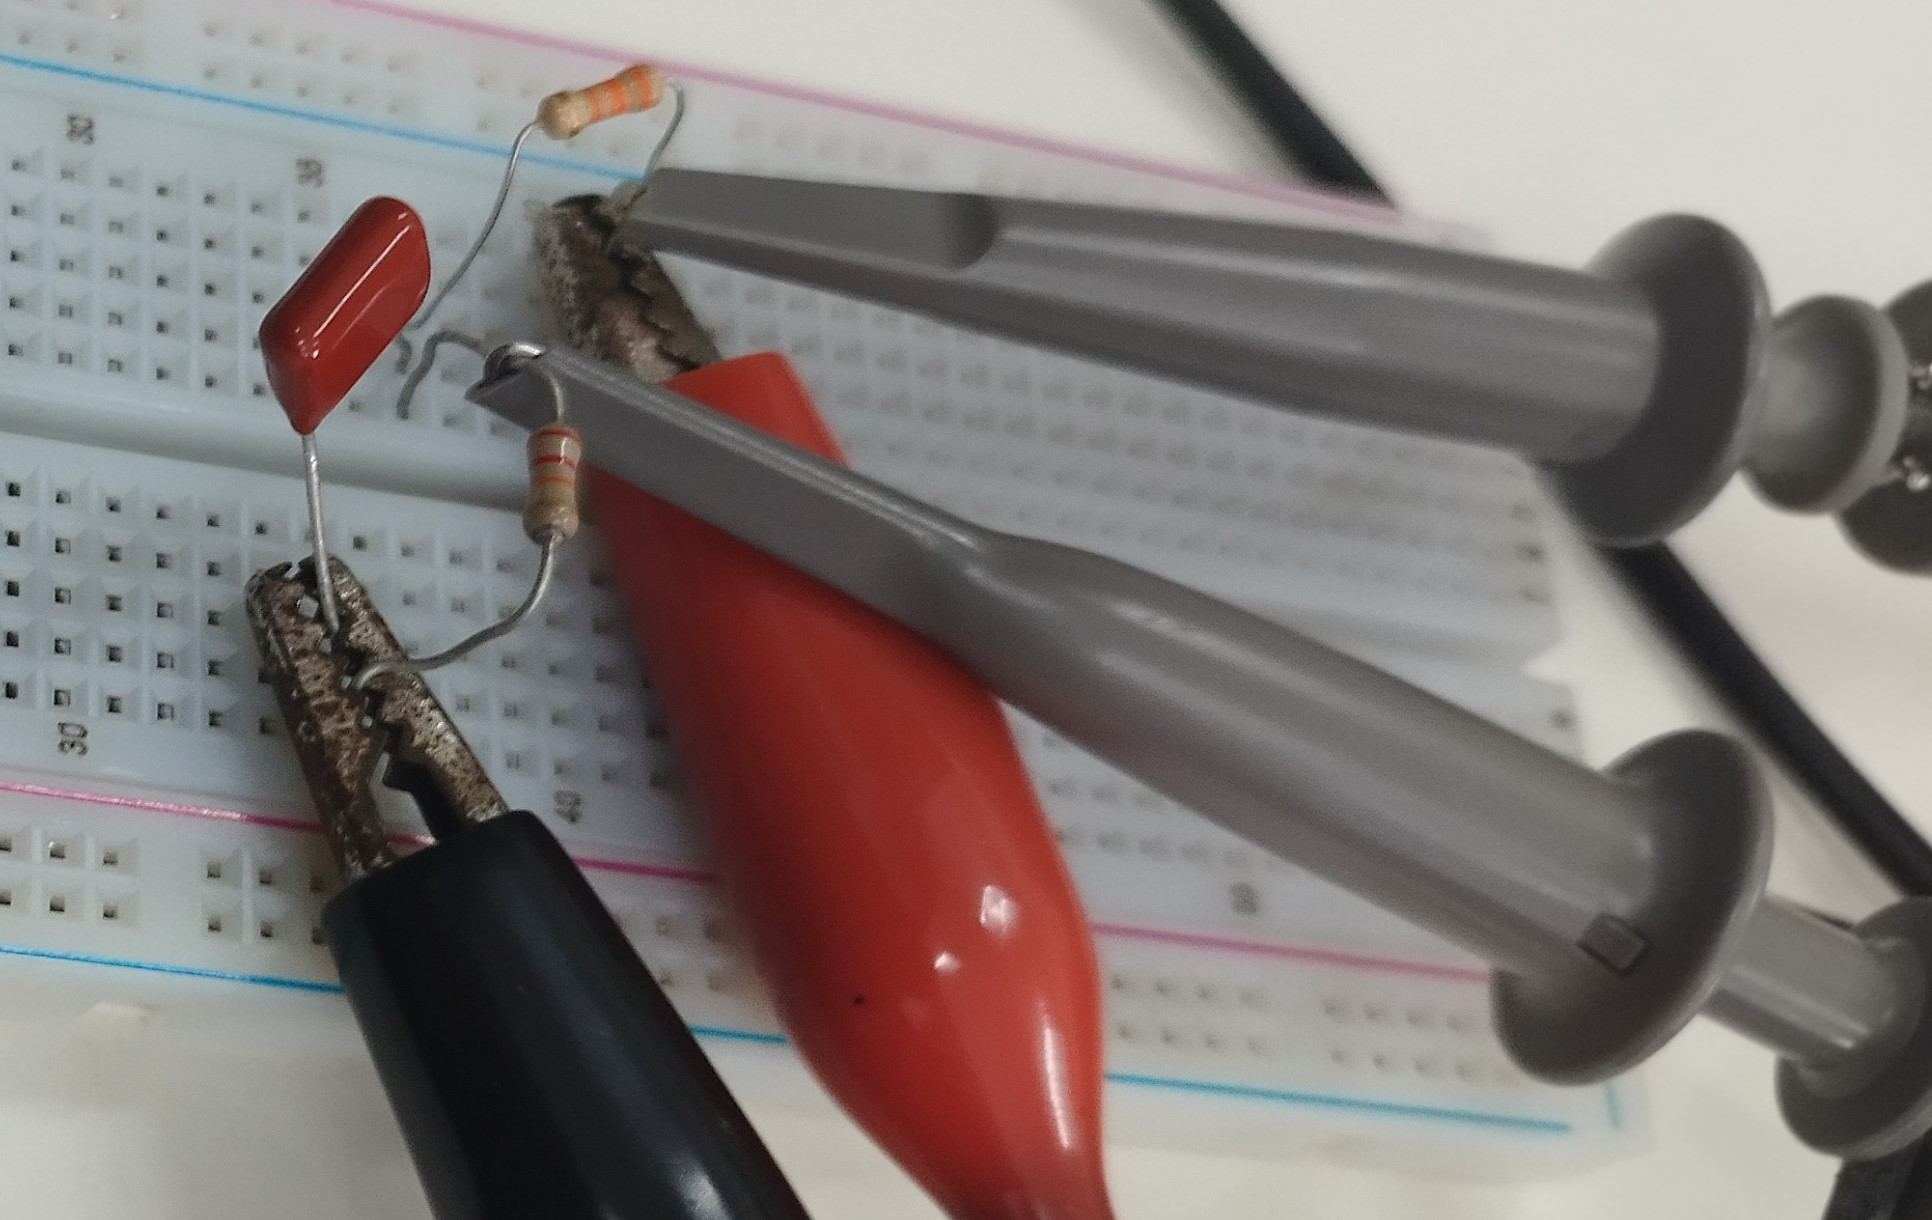
\includegraphics[width=0.6\textwidth]{imgs/protoboard_circuit2.jpg}
    \caption{Segundo circuito montado na protoboard.}
    \label{fig:protoboard_circuit2}
\end{figure}

\subsection{Configuração do Osciloscópio}

O gerador de sinal do osciloscópio será conectado na entrada \( v_i(t) \) do circuito. O gerador será configurado para gerar uma onda senoidal de amplitude de 5 V pico a pico e a frequência será ajustada para a mínima disponível de 100 mHz para observar a máxima tensão de saída que o filtro passa-baixa pode oferecer nas frequências baixas.

\begin{figure}[H]
    \centering
    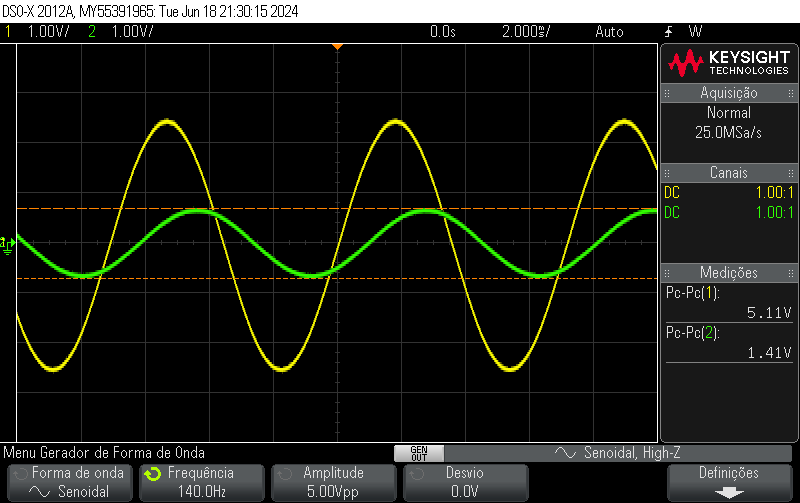
\includegraphics[width=0.7\textwidth]{imgs/second_oscilloscope_low_frequency_output.jpg}
    \caption{Curva de saída no osciloscópio para a frequência mínima de 100 mHz.}
    \label{fig:second_low_frequency_output}
\end{figure}

\subsection{Cálculo da Tensão Máxima}

Com base na máxima tensão de saída observada de 2,09 V, o valor de \( H_{\text{max}} \) é calculado da seguinte forma:

\begin{equation}
H_{\text{max}} = \frac{1}{\sqrt{2}} \times 2.09 \approx 1.478 \text{V}
\end{equation}

Este valor será utilizado para análises adicionais.

\subsection{Frequência de Corte Observada}
A frequência de corte observada, onde a amplitude de saída cai para 70.7\% da amplitude máxima observada, foi determinada como 140 Hz (ver Figura \ref{fig:second_oscilloscope_cutoff_frequency}. Esta informação é essencial para validar a performance do filtro em atenuar frequências acima deste ponto.

\begin{figure}[H]
    \centering
    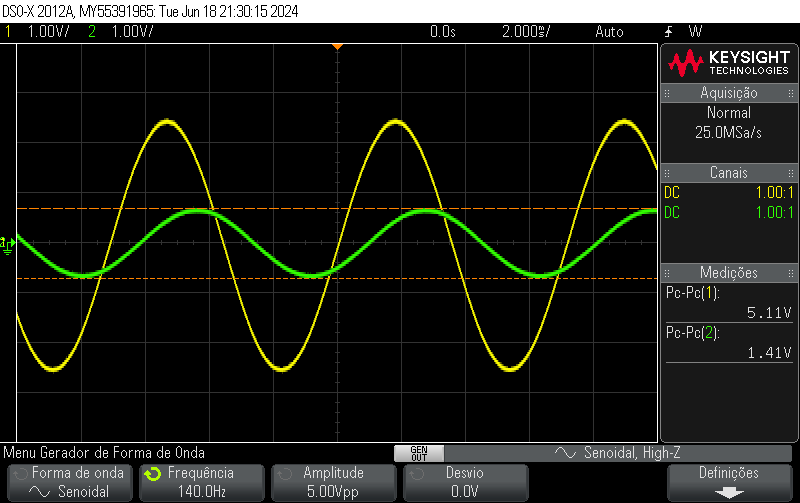
\includegraphics[width=0.7\textwidth]{imgs/second_oscilloscope_cutoff_frequency.jpg}
    \caption{Curva de saída no osciloscópio mostrando a frequência de corte para o Segundo Circuito.}
    \label{fig:second_oscilloscope_cutoff_frequency}
\end{figure}
\subsection{Cálculo da Tensão Máxima}


\subsection{Medição de Amplitudes em Frequências Variadas}

A amplitude de saída será medida para diferentes frequências para avaliar a frequência de corte do filtro. As amplitudes de entrada e saída para cada frequência testada serão registradas na seguinte tabela:

\begin{table}[H]
    \centering
    \begin{tabular}{|c|c|c|}
        \hline
        Frequência (Hz) & Amplitude de Entrada (Vi) & Amplitude de Saída (Vo) \\
        \hline
        100 m & 5.11 V & 2.09 V \\
        3 & 5.11 V & 2.05 V \\
        29.4 & 5.11 V & 2.01 V \\
        73.5 & 5.11 V & 1.81 V \\
        110.3 & 5.11 V & 1.57 V \\
        140 & 5.11 V & 1.41 V \\
        183.75 & 5.11 V & 1.21 V \\
        235.2 & 5.11 V & 1.01 V \\
        365.6 & 5.11 V & 760 mV \\
        514.5 & 5.11 V & 600 mV \\
        735 & 5.11 V & 440 mV \\
        1470 & 5.11 V & 280 mV \\
        2940 & 5.11 V & 200 mV \\
        \hline
    \end{tabular}
    \caption{Amplitudes de entrada e saída para diferentes frequências no circuito 2}
    \label{tab:second_frequency_response}
\end{table}

Este procedimento assegura uma compreensão detalhada da característica passa-baixa do filtro e da influência da frequência sobre a amplitude do sinal.

\section{Terceiro Circuito}

\subsection{Montagem do Circuito na Protoboard}

O circuito será montado na protoboard. Após a montagem, a fonte de tensão será conectada para alimentar o circuito. A figura abaixo mostra o circuito montado na protoboard.

\begin{figure}[H]
    \centering
    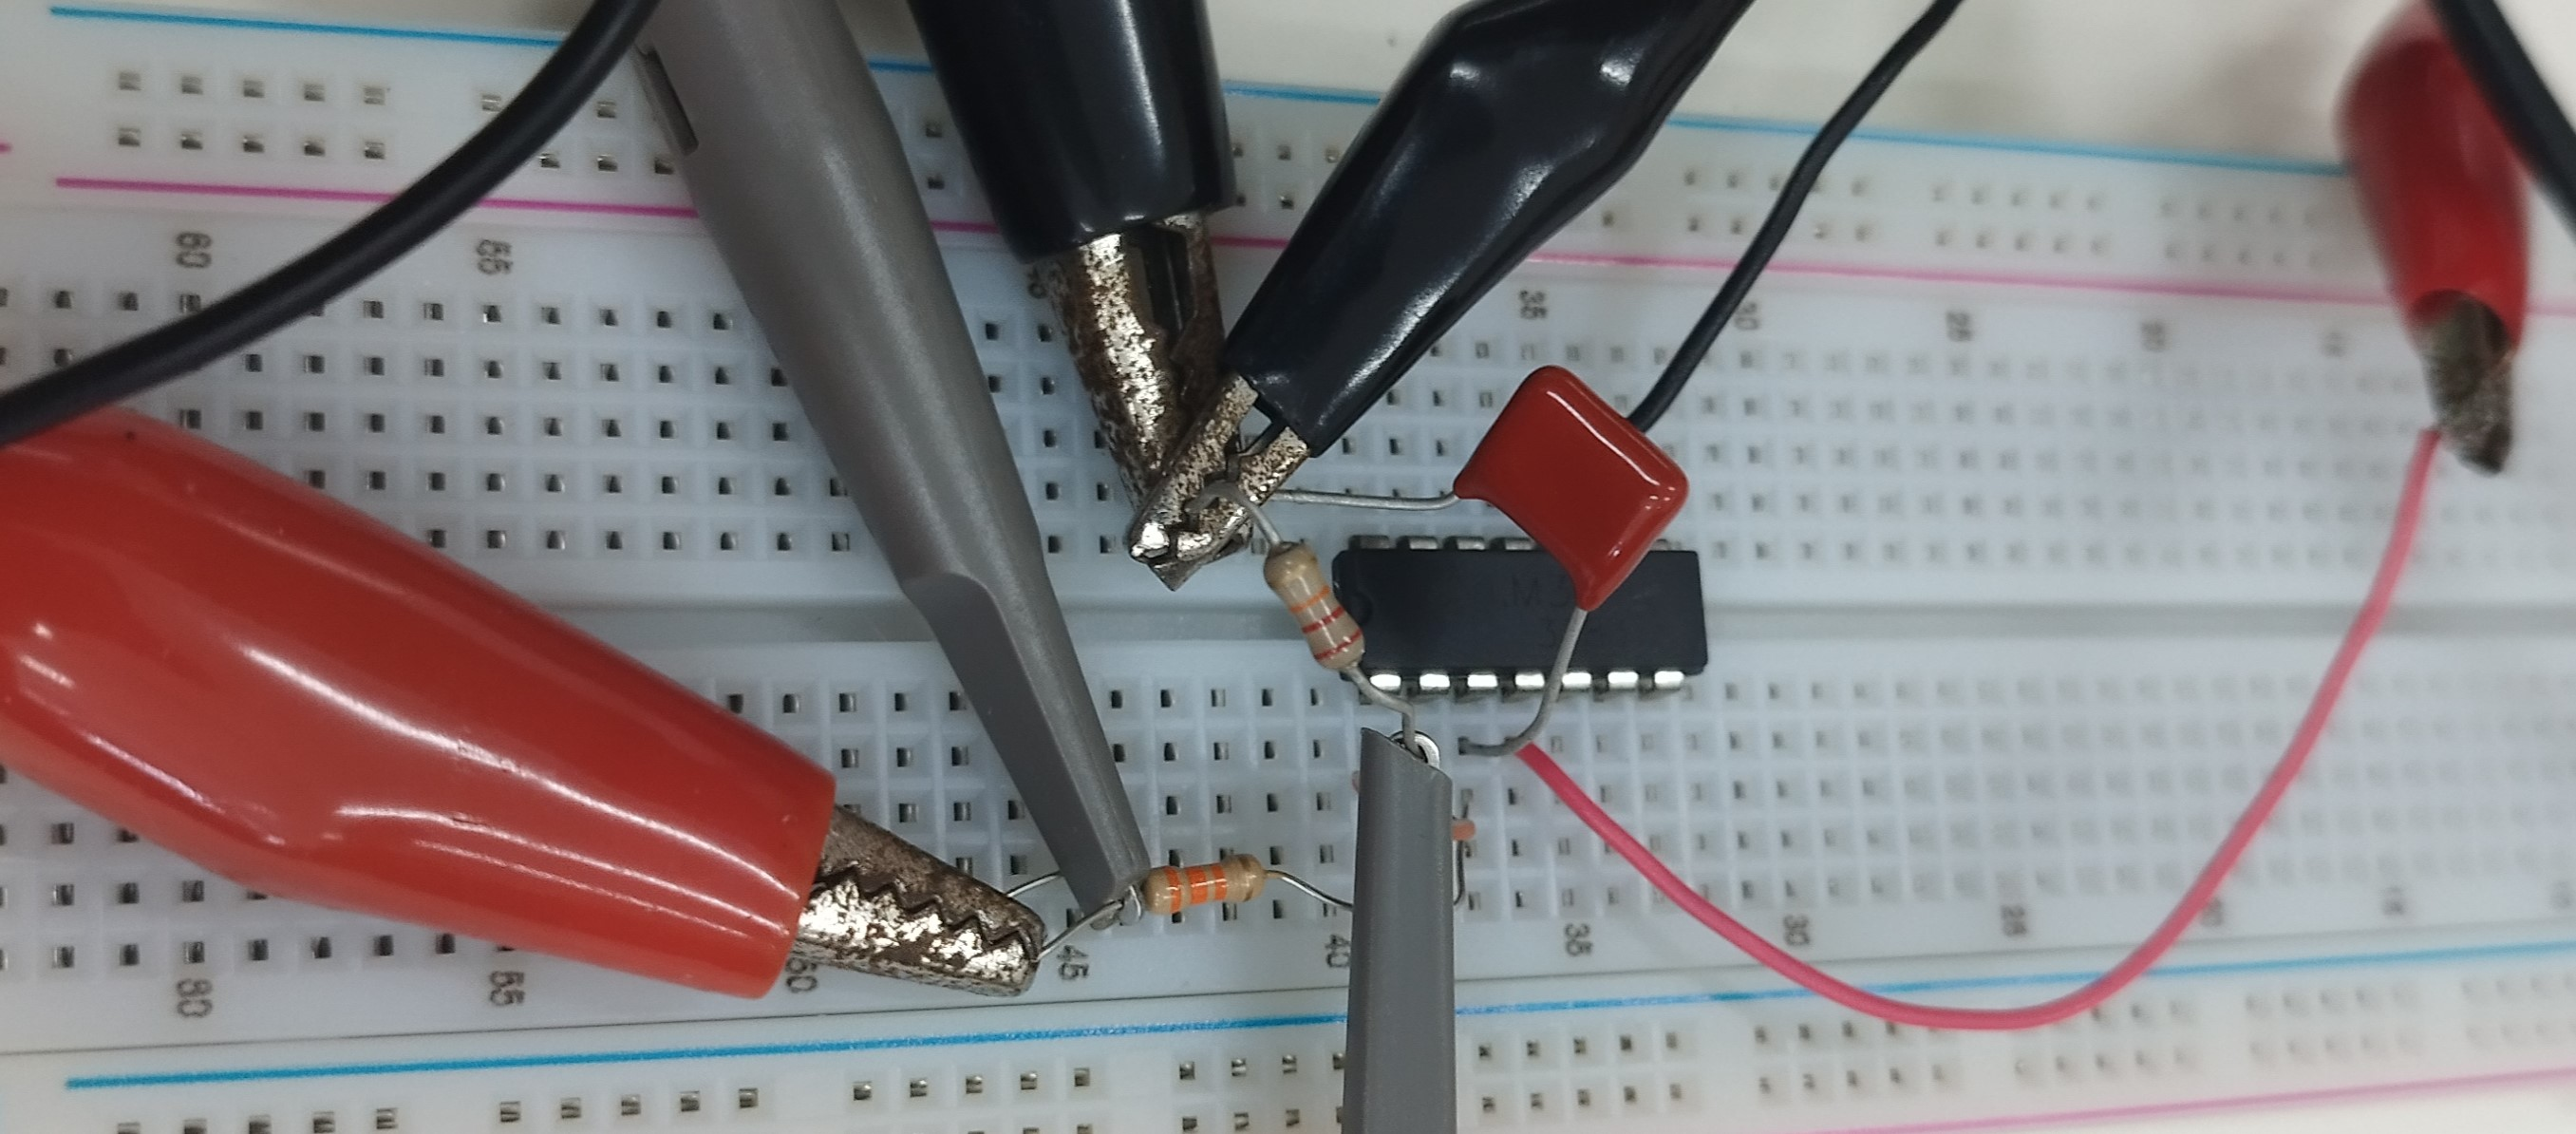
\includegraphics[width=0.7\textwidth]{imgs/protoboard_circuit3.jpg}
    \caption{Terceiro circuito montado na protoboard.}
    \label{fig:protoboard_circuit3}
\end{figure}

\subsection{Configuração do Osciloscópio}

O gerador de sinal do osciloscópio será conectado na entrada \( v_i(t) \) do circuito. O gerador será configurado para gerar uma onda senoidal de amplitude de 5 V pico a pico e a frequência será ajustada para a mínima disponível de 100 mHz para observar a máxima tensão de saída que o filtro passa-baixa pode oferecer nas frequências baixas.

%\begin{figure}[H]
%    \centering
%    \includegraphics[width=0.7\textwidth]%{imgs/third_oscilloscope_low_frequency_output.jpg}
    %\caption{Curva de saída no osciloscópio para a frequência mínima de 100 mHz.}
    %\label{fig:third_low_frequency_output}
%\end{figure}%


\subsection{Cálculo da Tensão Máxima}

Com base na máxima tensão de saída observada de 5.03 V, o valor de \( H_{\text{max}} \) é calculado da seguinte forma:

\begin{equation}
H_{\text{max}} = \frac{1}{\sqrt{2}} \times 5.03 \approx 3.56 \text{V}
\end{equation}

Este valor será utilizado para análises adicionais.

\subsection{Frequência de Corte Observada}
A frequência de corte observada, onde a amplitude de saída cai para 70.7\% da amplitude máxima observada, foi determinada como 43 Hz. Esta informação é essencial para validar a performance do filtro em atenuar frequências acima deste ponto.

\begin{figure}[H]
    \centering
    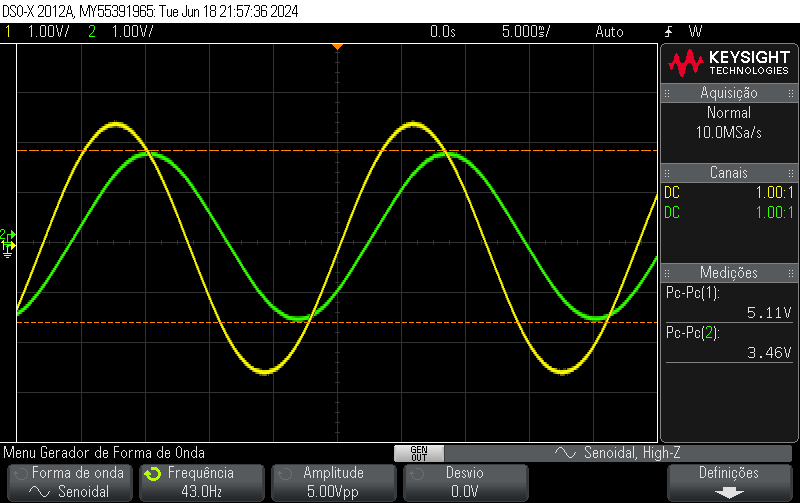
\includegraphics[width=0.7\textwidth]{imgs/third_oscilloscope_cutoff_frequency.jpg}
    \caption{Curva de saída no osciloscópio mostrando a frequência de corte para o Terceiro Circuito.}
    \label{fig:third_oscilloscope_cutoff_frequency}
\end{figure}


\subsection{Medição de Amplitudes em Frequências Variadas}

A amplitude de saída será medida para diferentes frequências para avaliar a frequência de corte do filtro. As amplitudes de entrada e saída para cada frequência testada serão registradas na seguinte tabela:

\begin{table}[H]
    \centering
    \begin{tabular}{|c|c|c|}
        \hline
        Frequência (Hz) & Amplitude de Entrada (Vi) & Amplitude de Saída (Vo) \\
        \hline
        100 m & 5.11 V & 5.03 V \\
        900 m & 5.11 V & 4.46 V \\
        8.6 & 5.14 V & 4.38 V \\
        21.5 & 5.11 V & 4.14 V \\
        32.3 & 5.11 V & 3.86 V \\
        43 & 5.11 V & 3.5 V \\
        53.8 & 5.11 V & 3.38 V \\
        68.8 & 5.11 V & 2.93 V \\
        107.5 & 5.11 V & 1.81 V \\
        150.5 & 5.11 V & 1.33 V \\
        215 & 5.11 V & 1.01 V \\
        430 & 5.11 V & 520 mV \\
        860 & 5.11 V & 320 mV \\
        \hline
    \end{tabular}
    \caption{Amplitudes de entrada e saída para diferentes frequências no circuito 3}
    \label{tab:third_frequency_response}
\end{table}

Este procedimento assegura uma compreensão detalhada da característica passa-baixa do filtro e da influência da frequência sobre a amplitude do sinal.


\chapter{Resultados}

Os resultados obtidos a partir das medições laboratoriais, teóricas e simulações revelam comportamentos característicos dos filtros passa-baixas implementados nos três circuitos analisados. A análise focalizou-se na avaliação das frequências de corte, na máxima tensão de saída e na forma como esses elementos se alinham com as previsões teóricas das funções de transferência.

\section{Características Observadas nos Circuitos}

Os três circuitos exibiram a propriedade fundamental de um filtro passa-baixas, que é a manutenção da máxima tensão de saída em frequências baixas. Como foi teoricamente previsto e confirmado pelas simulações e medições em laboratório, a amplitude da saída diminui conforme a frequência de entrada excede a frequência de corte. Esta característica foi visualmente confirmada pelos gráficos de Bode (ver Figuras \ref{fig:first_circuit_ltspice_bode}, \ref{fig:second_circuit_ltspice_bode}, e \ref{fig:third_circuit_ltspice_bode}), que mostraram uma queda na resposta de ganho próximo às respectivas frequências de corte de cada filtro.

\subsection{Análise das Funções de Transferência}

As funções de transferência dos três circuitos, detalhadas nas equações \ref{eq:first_transfer_function} e \ref{eq:second_transfer_function}, fundamentam o comportamento observado. No caso dos circuitos primeiro e terceiro, as frequências de corte foram semelhantes, o que indica uma similaridade nas características dos componentes de design, apesar de variações mínimas nos valores componentes. Em contraste, o segundo circuito apresentou uma frequência de corte significativamente diferente, devido a variações na configuração de seus elementos (ver Figura \ref{fig:second_oscilloscope_cutoff_frequency}).

\subsection{Comparação das Frequências de Corte}

Interessante observar que, apesar de variações nas frequências de corte observadas entre o primeiro e o segundo circuito, a consistência do desempenho dentro dos parâmetros de um filtro passa-baixas se manteve. A frequência de corte do segundo circuito (\( f_{c2} \)) foi diferente devido às diferenças nas funções de transferência e nos valores componentes utilizados. Esta observação destaca a importância de escolher apropriadamente os componentes durante o design para atender às especificações desejadas.

\section{Síntese dos Resultados}

Os dados consolidados oferecem uma visão ampla da eficácia dos designs de filtro e da adequação das técnicas de simulação e medição. As análises teóricas se alinham bem com as observações práticas, o que confirma a validade dos modelos teóricos utilizados e proporciona uma base sólida para futuras iterações de design e optimização.


\chapter{Conclusão}

Esta atividade validou a eficácia dos filtros passa-baixas, confirmando a consistência entre teoria, simulações e resultados experimentais. Três diferentes circuitos foram investigados, todos aderindo ao princípio fundamental de maximizar a tensão de saída em frequências baixas e atenuar as altas. 

As análises realizadas demonstram que simulações e medições são métodos eficazes para validar a performance dos filtros. Além disso, recomenda-se a realização de pesquisas adicionais para explorar o impacto de variáveis externas, como a temperatura, no desempenho dos filtros a longo prazo.

Portanto, este estudo enfatiza a importância de métodos de simulação e medição precisos para o desenvolvimento e validação de componentes eletrônicos, servindo como um guia prático para futuras inovações na engenharia eletrônica.




\clearpage
\bibliography{bibliografia}



\end{document}

% ----------------------------------------------------------
% ELEMENTOS PÓS-TEXTUAIS
% ----------------------------------------------------------
\postextual

% ----------------------------------------------------------
% Referências bibliográficas
% ----------------------------------------------------------
\bibliography{bibliografia}

% ----------------------------------------------------------
% Glossário
% ----------------------------------------------------------
%
% Consulte o manual da classe abntex2 para orientações sobre o glossário.
%
%\glossary



\end{document}
